\section{負荷についての実験}
%%%%%%%%%%%%%%%%%%%%%%%%%%%%%%%%%%
%    実験の目的
%%%%%%%%%%%%%%%%%%%%%%%%%%%%%%%%%%
\subsection{実験の目的}
そこで, Differential Syncronizationに基づいた, 本研究の同期機構が大量のリクエストに対して, どの程度影響が出るか確かめる.
%%%%%%%%%%%%%%%%%%%%%%%%%%%%%%%%%%
%    実験環境
%%%%%%%%%%%%%%%%%%%%%%%%%%%%%%%%%%
\subsection{実験環境}
本手法を実現するサーバとクライアントを実装する. 本実験使用したサーバの計算機環境を表\ref{server}に示す. また2つのクライアントの計算機環境を表\ref{client1}, 表\ref{client2}に示す.
% ネットワーク
\begin{table}[htbp]
\begin{center}
	\caption{使用するサーバのスペック}
	\begin{tabular}{|l|l|} \hline
		OS &  macOS Sierra \\ \hline
		CPU & Intel(R) Core(TM) i5-5250U CPU 1.6GHz \\ \hline
		メモリ & 8GB \\ \hline
    開発言語 & Ruby \\ \hline
		データベース & MySQL \\ \hline
		Webサーバ & Puma\\ \hline
	\end{tabular}
	\label{server}
\end{center}
\end{table}

\begin{table}[htbp]
\begin{center}
	\caption{使用するクライアント1のスペック}
	\begin{tabular}{|l|l|} \hline
		OS & macOS Sierra \\ \hline
		CPU & Intel(R) Core(TM) i5-5250U CPU 1.6GHz \\ \hline
		メモリ & 8GB \\ \hline
    開発言語 & JavaScript HTML \\ \hline
	\end{tabular}
	\label{client1}
\end{center}
\end{table}

\begin{table}[htbp]
\begin{center}
	\caption{使用するクライアント2のスペック}
	\begin{tabular}{|l|l|} \hline
		OS & macOS Sierra \\ \hline
		CPU & Intel(R) Core(TM) i5-5250U CPU 1.6GHz \\ \hline
		メモリ & 8GB \\ \hline
    開発言語 & JavaScript HTML \\ \hline
	\end{tabular}
	\label{client2}
\end{center}
\end{table}

%%%%%%%%%%%%%%%%%%%%%%%%%%%%%%%%%%
%    実験方法
%%%%%%%%%%%%%%%%%%%%%%%%%%%%%%%%%%
\subsection{実験方法}
クライアントを2つ用意した.
クライアント1から命令を発行し, 同期レスポンス時間を計測した.
クライアント1がサーバに差分をリクエストした時刻からレスポンスが届いた時刻までを同期レスポンス時間と定義した.
また, クライアントは4秒ごとにサーバにリクエストを送信した. その間, クライアント2では通常の同期を行なった.
2パターンの計測を行った.
まず, (1)クライアント1は40秒間4秒ごとに面を作る命令を送信した. 面を作る命令の数を4秒ごとに倍にしていき, 同期レスポンス時間の計測を行った. 最初の面を作成する数は1個とした. 同期レスポンス時間が2分を超え同期に遅延が生じたと判断できるところで計測を終了した.
次に, (2)クライアント1は4秒ごとに, 40個の面を作成する命令を, (1)で計測不能になるまで作成した面の数になるまで送信した. それまでのクライアント1の同期レスポンス時間を計測した.

%%%%%%%%%%%%%%%%%%%%%%%%%%%%%%%%%%
%    実験結果
%%%%%%%%%%%%%%%%%%%%%%%%%%%%%%%%%%
\subsection{実験結果}
(1)の計測による, クライアント1での同期レスポンス時間の計測した結果を図\ref{jikken3}に示す.
項目は左から送信するデータの大きさ, 同期レスポンス時間, 同期レスポンス時間を表したタイムラインである. 計測の結果, 命令の数が増えるとデータの大きさが大きくなり, 同期レスポンス時間が増える.
\begin{figure}[htbp]
 \begin{center}
	 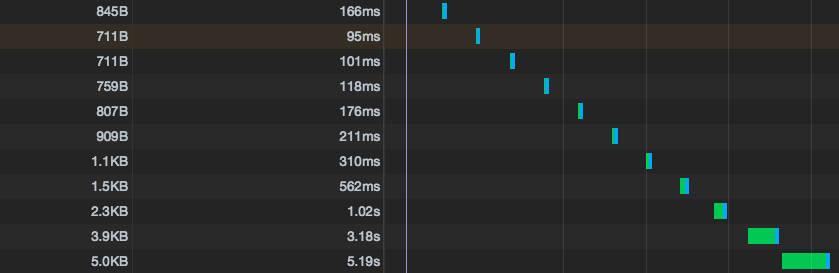
\includegraphics[scale=0.5]{images/jikken3}
	 \caption{(1)の計測による同期レスポンス時間}
	 \label{jikken3}
 \end{center}
\end{figure}
(1)の計測で, 面が500個作成されたところで終了した. よって(2)は面が500を超えるまで計測を続けた.
(2)の計測による, クライアント1での同期レスポンス時間の計測した結果を図\ref{jikken2}に示す.
計測の結果, 一度に大量のリクエストでなければ, たくさんの面を扱うことができる.
\begin{figure}[htbp]
 \begin{center}
	 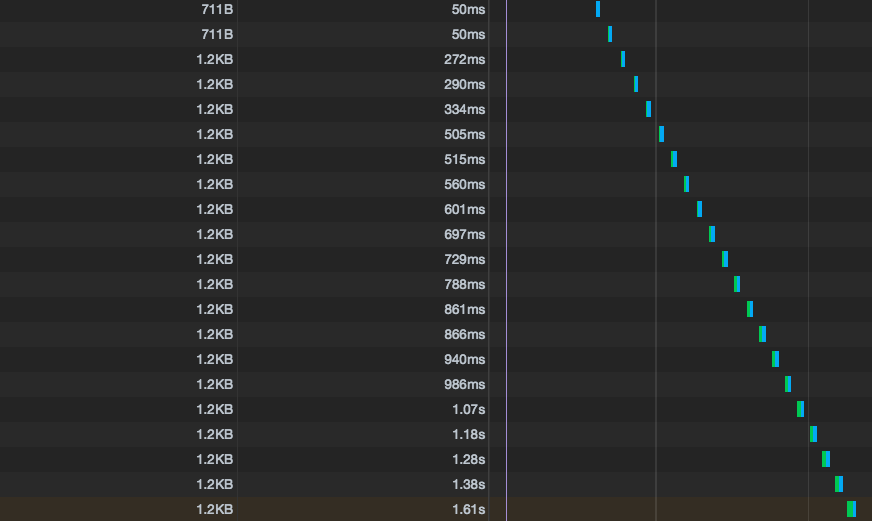
\includegraphics[scale=0.5]{images/jikken2}
	 \caption{(2)の計測による同期レスポンス時間}
	 \label{jikken2}
 \end{center}
\end{figure}
%%%%%%%%%%%%%%%%%%%%%%%%%%%%%%%%%%
%    考察
%%%%%%%%%%%%%%%%%%%%%%%%%%%%%%%%%%
\subsection{考察}
結果より, 面を作る数が増え, 一度に大量の編集命令がサーバにリクエストされた場合, サーバにとって負荷となる.
また, 命令を分散させて送信すれば, 本システムは問題なく同期サイクルを回すことができる.
以上より, サーバでの適用や差分の計算に要する時間が多くかかっていることがわかり, 原因として, データベースでの挿入や検索がボトルネックになっていると考えられる.
